
\lecture{Binomial Random Variables}{binomial-random-variables}
\part{Binomial Random Variables}

\title{Binomial Random Variables}
\subtitle{Counting Events}

\author{Kelly Black}
\institute{Clarkson University}
\date{10 Feb 2012}

\begin{frame}
  \titlepage
\end{frame}

\begin{frame}
  \frametitle{Outline}
  \tableofcontents[pausesection,hideallsubsections,part=1]
\end{frame}


\section{Clicker Quiz}


\begin{frame}
  \frametitle{Clicker Quiz}

  You are going to flip a coin four times. What is the probability of
  getting three tails?

    \vfill

  \begin{tabular}{l@{\hspace{3em}}l@{\hspace{3em}}l}
    A: 1/4 & B: 1/2 & C: 3/4
  \end{tabular}

  \vfill
  \vfill
  \vfill


\end{frame}


\begin{frame}{Turn It Around}

  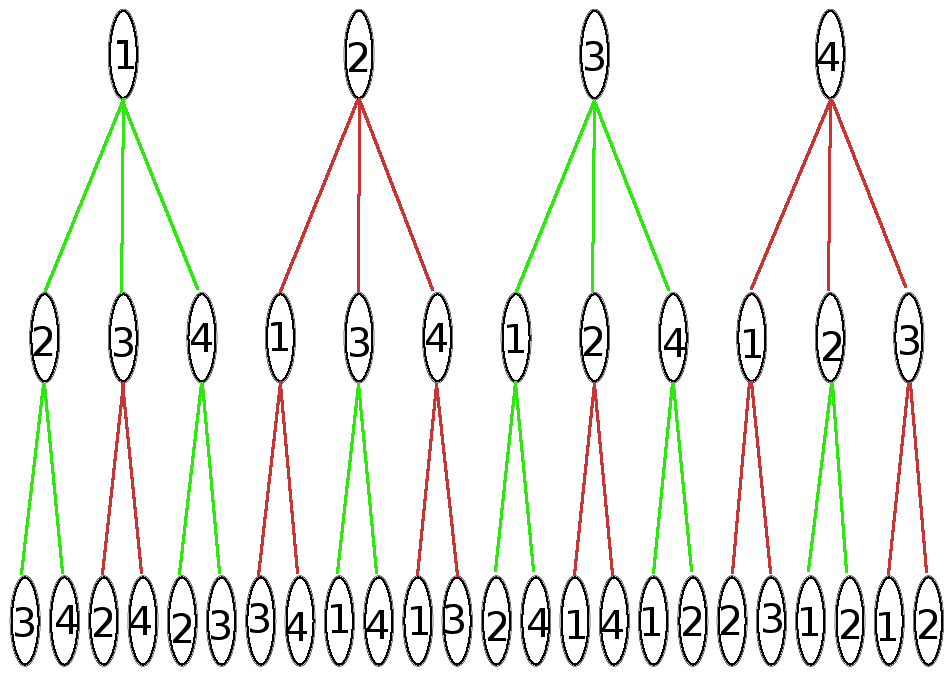
\includegraphics[width=11cm,height=6cm]{img/binomialTree}
  
\end{frame}



\section{Examples}

\begin{frame}
  \frametitle{Example}

  It is estimated that in a given monthly period 55\% od all stocks
  will rise. I pick four stocks at random (with replacement). What is
  the probability that I get exactly one stock that rises?

  \vfill

\end{frame}


\begin{frame}
  \frametitle{Example}

  It is estimated that 2\% of the shirts made at a factory are not
  suitable for sale. You choose 20 shirts at random (with
  replacement). What is the probability that you find exactly three
  unsuitable shirts?

  \vfill

\end{frame}

\begin{frame}{Clicker Quiz}

  A basketball player has a lifetime average of making 60\% of his
  free throws. In a particular game he will attempt ten free
  throws. What is the probability that he will make exactly six free
  throws?

    \vfill

  \begin{tabular}{l@{\hspace{3em}}l@{\hspace{3em}}l@{\hspace{3em}}l}
    A: .20 & B: .25 & C: .50 & D: .60
  \end{tabular}

  \vfill
  \vfill
  \vfill
  
\end{frame}


% LocalWords:  Clarkson pausesection hideallsubsections
